% =============================================
% ==           sections/intro.tex            ==
% =============================================
\section{Introduction}\label{sec:intro}

% --- Introduction to Environment and MARL Challenges ---
A multi-agent system~\cite{weissMultiagentSystems2016} consists of a collection of autonomous, interacting entities that operate within a shared environment, which they observe through sensors and influence through actuators~\cite{busoniuComprehensiveSurveyMultiagent2008a}.
Multi-agent systems (MAS) have become a decisive framework for solving a series of complex real-world problems, offering a scalable, robust, and highly adaptive approach~\cite{messingIntroductionMultiAgentSystems2002}.
The application of multi-agent systems spans a wide range of fields, such as distributed control,robotics, resource management, collaborative decision-making,etc.~\cite{critesElevatorGroupControl1998,riedmillerReinforcementLearningCooperating2001,tesauroPricingAgentEconomies2002,steingroverReinforcementLearningTraffic2005}
Furthermore, the domain of artificial intelligence for gaming has served as a crucial testbed, with agents demonstrating sophisticated, team-based strategies in complex environments like StarCraft II and Dota 2, often surpassing the world's best human players~\cite{vinyalsGrandmasterLevelStarCraft2019,openaiDota2Large2019}.
Despite these successes, the core difficulty in designing agent policies stems from the non-stationarity of the environment: from any single agent's perspective, the world is constantly changing as other agents simultaneously learn and adapt their strategies~\cite{stoneMultiagentSystemsSurvey2000}.
To address this, Multi-Agent Reinforcement Learning (MARL) has emerged as the leading paradigm for enabling agents to autonomously learn complex cooperative policies.

Jointly released by DeepMind and Blizzard, StarCraft~II (SC2) is a prominent benchmark 
for multi-agent cooperation research, attributed to its challenging characteristics, 
including partial observability, vast action and state spaces, and long-term delayed rewards.
XuanCe is an open-source deep reinforcement learning library featuring a modular design 
that provides a rich repository of both single-agent and multi-agent algorithms~\cite{liuXuanCeComprehensiveUnified2023}. 
The integration of XuanCe with the SC2 environment simulates complex cooperative scenarios, 
establishing an ideal testbed for our experimental evaluation.

\begin{figure*}[htbp]
    \centering %
    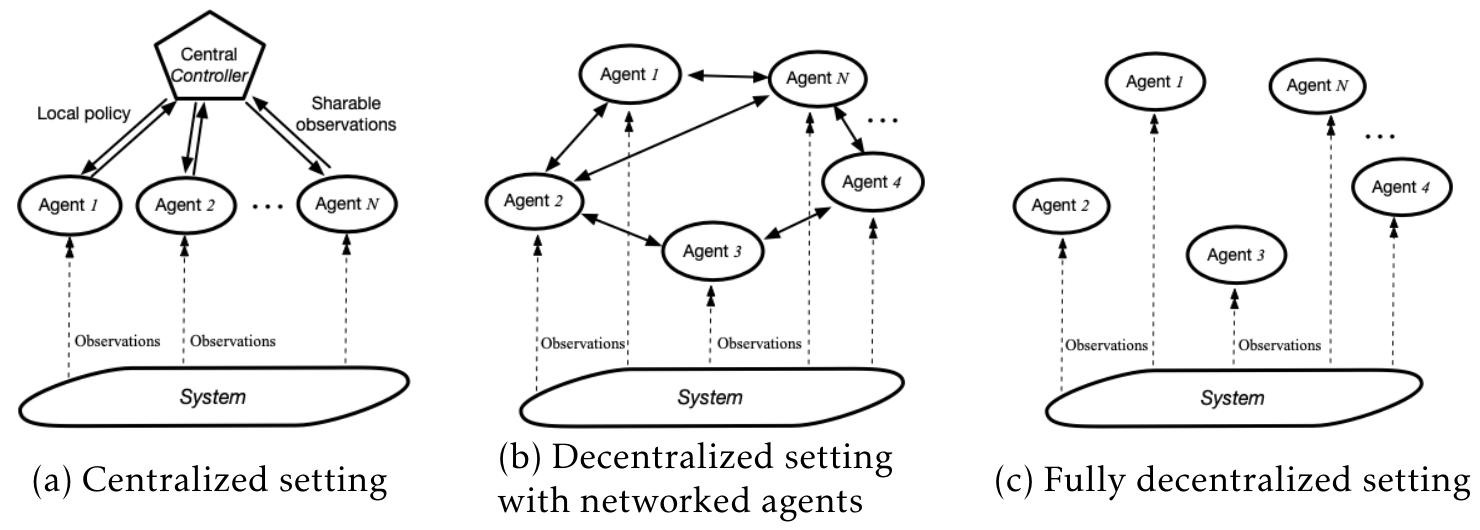
\includegraphics[width=0.8\textwidth]{Three different information structures.jpeg}
    \caption{
        In (a), a central controller uses global information to create and distribute policies (e.g., CTDE). This structure simplifies analysis in cooperative tasks but is unsuitable for non-cooperative ones.
        In (b), agents exchange information locally with neighbors without a central controller. This poses an intermediate challenge for theoretical analysis.
        In (c), Agents act independently using only local observations, with no communication. This is the most difficult to analyze, as it requires aligning local decisions with a global objective.
        Adapted from Fig.~2 in~\cite{zhangMultiAgentReinforcementLearning2021}, caption revised
    }\label{fig:Three different information structures}
\end{figure*}
Despite advancements in multi-agent reinforcement learning (MARL), the field still grapples with fundamental challenges that hinder its theoretical rigor and practical scalability:
(1)~\textbf{Non-Unique Learning Goals}, which arise from misaligned agent objectives and lead to ambiguous performance criteria—ranging from converging to Nash equilibria (under full rationality assumptions) to optimizing auxiliary goals like communication efficiency or robustness, complicating the definition of ``optima'' learning outcomes;
(2)~\textbf{Non-Stationarity}, where concurrent policy updates across agents render the environment dynamically changing, violating the stationary Markovian property critical to single-agent RL analyses and often causing independent learning strategies to fail in convergence;
(3)~\textbf{Scalability Issue}, driven by the exponential growth of the joint action space with the number of agents (the ``combinatorial nature''),  which dramatically increases the difficulty of theoretical analysis, especially convergence analysis;\@
and (4)~\textbf{Various Information Structures}, where agents typically only access local observations instead of global state/policy information, exacerbating non-stationarity and increasing the difficulty of aligning local decisions with global team objectives across centralized, networked, or fully decentralized settings (shown in Fig.~\ref{fig:Three different information structures})\cite{zhangMultiAgentReinforcementLearning2021}.
To address these issues, several technical paradigms have emerged:
\begin{enumerate}
    \item \textbf{Value Function Decomposition:} Represented by algorithms such as QMIX and its weighting schemes: Centrally-Weighted (CW) QMIX and Optimistically-Weighted (OW) QMIX, this approach decomposes the global team value function ($Q_{\text{tot}}$) into a sum or a more complex combination of individual agent value functions ($Q_i$).

    \item \textbf{Actor-Critic Methods:} These methods decouple policy learning (the Actor) from value estimation (the Critic) and are ingeniously extended under the Centralized Training with Decentralized Execution (CTDE) framework. They can be further subdivided into off-policy (e.g., MADDPG) and on-policy (e.g., MAPPO) approaches.

    \item \textbf{Fully Decentralized Methods:} This paradigm forgoes centralized training, where each agent learns independently by treating all other agents as part of the environment. Representative algorithms in this category include Independent PPO (IPPO) and Independent Q-Learning (IQL).
\end{enumerate}

% --- Motivation and Core Research Focus ---

Among these, MAPPO, a multi-agent extension of PPO, excels within the Centralized Training, 
Decentralized Execution (CTDE) framework and has recently achieved SOTA results on several benchmarks. 
Its framework offers a mainstream solution to MARL's challenges by aggregating global information 
during training while relying on local observations during execution.
Therefore, this paper aims to investigate the underlying reasons for MAPPO's effectiveness 
in mitigating these challenges, explore its applicable scenarios, and identify potential avenues for further algorithmic refinement. 
To this end, we conduct a systematic performance evaluation of four algorithms---MAPPO, QMIX, OW-QMIX and IPPO---on the StarCraft~II platform within XuanCe. 
This investigation, which forms the core of our research, is designed to reveal MAPPO's performance advantages, 
operational boundaries, and underlying mechanisms in various cooperative scenarios.

% --- Main Contributions ---

The main contributions of this paper are as follows:
\begin{itemize}
    \item We conduct a comparison of four algorithms---MAPPO, QMIX, OW-QMIX
    and IPPO---in multi-agent cooperative scenarios built upon the integration of the XuanCe library and the SC2 platform. 
    The evaluation is based on key metrics including task win rate, policy convergence speed, and training stability.

    \item We elucidate the underlying mechanisms of MAPPO's performance advantages, providing instructive 
    guidance for the selection of the MAPPO algorithm in practical applications.
\end{itemize}